
\section{Ilustrando a PR}

%%{\bf \textcolor{red}{Vou refazer novos desenhos... aguardem}}

 O objetivo destes problemas é ilustrar o paradigma da PR.
Para cada uma das ilustrações que se seguem,
construa um programa que retorne o número de pontos válidos na implementação 
de seu modelo. O domínio da variável $x$ e $y$ são inteiros,
e tem seus limites dado pelas figuras.

Faça as suposições que julgares necessárias, visando as melhorias
deste problema e seu objetivo (acompanhe as aulas). Seu primordial
objetivo é ilustrar a PR via várias áreas do Espaço de Estados (EE) 
de um problema.



\subsection{O brasão da CroáXia}

 A CroáXia é um belo país, e tem uma bandeira
  um pouco bizarra, mas a parte marcante é são as cores do seu brasão, representando
  as duas etnias predominantes deste país. Assim, como todo aluno
  da CroáXia deve conhecer o brasão, lá eles usam o mesmo para ensinar matemática.
  Há bons matemáticos por lá, mas pediram ajuda para saber quais os pontos 
  na amostra abaixo e qual a área em vermelho.

 \begin{figure}[!ht]
  \centering
    %\reflectbox{%
      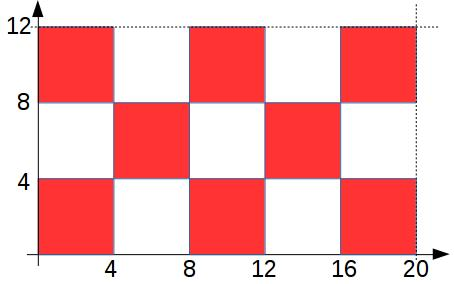
\includegraphics[width=0.5\textwidth , height=0.25\textheight]{croacia_flag.jpg}
      %%}
      \caption{Ilustrando a PR}
\label{fig_croacia}
\end{figure}

As áreas hachuradas da figura \ref{fig_croacia} são pontos válidos da solução,
logo, extremidades são contabilizadas como soluções válidas. Outro detalhe,
que algumas destas restrições, são fornecidas por funções tais como, por 
exemplo: $| x - y| \:\: mod \:\:  4$, logo, use-a.
O número de pontos ou soluções válidas
no Minizinc, são obtidas ao se habilitar as opções de \textit{verbose solving} 
e \textit{statitics for solving}, pois cada ponto válido é uma soluçao para este problema.



\subsection{Quais são os pontos no triângulo?}

Quais são os pontos da área definida pelo triângulo da figura \ref{fig_triangulo}?

 \begin{figure}[!ht]
  \centering
    %\reflectbox{%
      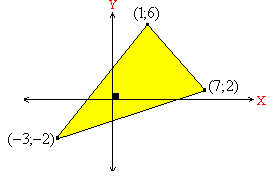
\includegraphics[width=0.5\textwidth , height=0.2\textheight]{triangulo_amarelo.png}
      %%}
      \caption{Ilustrando a PR}
\label{fig_triangulo}
\end{figure}
Basta imprimir os pontos válidos dentro desta área. O número de pontos ou soluções válidas
no Minizinc, são obtidas ao se habilitar as opções de \textit{verbose solving} e \textit{statitics for solving}, pois cada ponto válido é uma soluçao para este problema.





\subsection{Quais são os pontos? -- 01}
 Quais são os pontos definidos  pela área  da figura \ref{fig_area_validas01}?
 \begin{figure}[!h]
  \centering
    %\reflectbox{%
      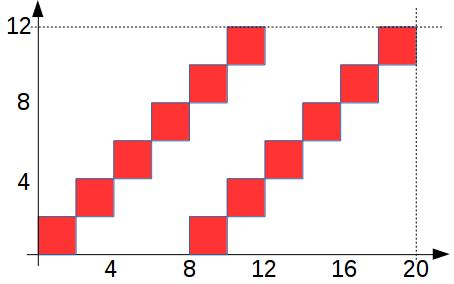
\includegraphics[width=0.5\textwidth , height=0.25\textheight]{area_validas01.jpg}
      %%}
      \caption{Ilustrando a PR}
\label{fig_area_validas01}
\end{figure}

Basta imprimir os pontos válidos dentro desta área. O número de pontos ou soluções válidas
no Minizinc, são obtidas ao se habilitar as opções de \textit{verbose solving} e \textit{statitics for solving}, pois cada ponto válido é uma soluçao para este problema.



\subsection{Quais são os pontos? -- 02}

 Quais são os pontos definidos  pela área da figura \ref{fig_area_validas02}?
 \begin{figure}[!ht]
  \centering
    %\reflectbox{%
      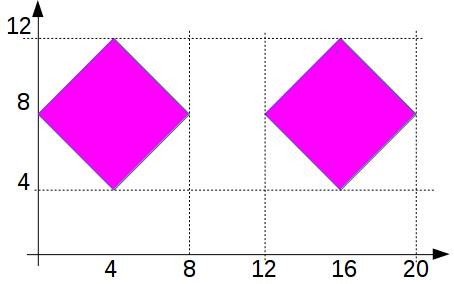
\includegraphics[width=0.5\textwidth , height=0.25\textheight]{area_validas02.jpg}
      %%}
      \caption{Ilustrando a PR}
\label{fig_area_validas02}
\end{figure}

Basta imprimir os pontos válidos dentro desta área. O número de pontos ou soluções válidas
no Minizinc, são obtidas ao se habilitar as opções de \textit{verbose solving} e \textit{statitics for solving}, pois cada ponto válido é uma soluçao para este problema.



\subsection{Quais são os pontos? -- 03}

Quais são os pontos definidos  pela área hachurada da figura \ref{fig_area_validas03}?
 \begin{figure}[!hb]
  \centering
    %\reflectbox{%
      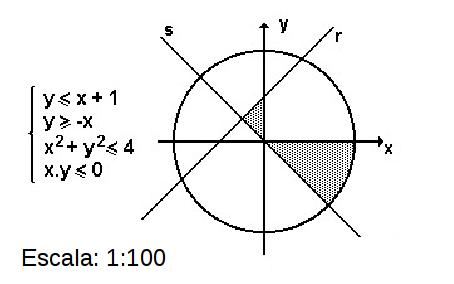
\includegraphics[width=0.5\textwidth , height=0.2\textheight]{area_validas03.jpg}
      %%}
      \caption{Refazer esta figura bem como as equações-- Escala 1:100 $x$ 100}
\label{fig_area_validas03}
\end{figure}


Basta imprimir os pontos válidos dentro desta área. O número de pontos ou soluções válidas
no Minizinc, são obtidas ao se habilitar as opções de \textit{verbose solving} e \textit{statitics for solving}, pois cada ponto válido é uma soluçao para este problema.

